\documentclass{article}

\usepackage[final,main]{neurips_2025}
\usepackage[utf8]{inputenc}
\usepackage[T1]{fontenc}
\usepackage{hyperref}
\usepackage{url}
\usepackage{booktabs}
\usepackage{amsfonts}
\usepackage{nicefrac}
\usepackage{microtype}
\usepackage{xcolor}
\usepackage{graphicx}
\usepackage{subcaption}
\usepackage{multirow}
\usepackage{array}
\usepackage{natbib}

% Remove NeurIPS footer notice
\makeatletter
\renewcommand{\@noticestring}{}
\makeatother

\title{From Conversion Crisis to Forecast:\\
  Analytics and Predictive Modeling for a Vietnamese Fashion E-Commerce Business}

\author{%
  \begin{tabular}{cc}
    \begin{minipage}[t]{0.45\textwidth}\centering
      To Gia Bao \\
      HCMUS \\
      \texttt{example@hcmus.edu.vn}
    \end{minipage} &
    \begin{minipage}[t]{0.45\textwidth}\centering
      Nguyen Le Lam Phuc \\
      HCMUS \\
      \texttt{example@hcmus.edu.vn}
    \end{minipage} \\[10pt]
    \begin{minipage}[t]{0.45\textwidth}\centering
      Phan Van Hoang \\
      HCMUS \\
      \texttt{example@hcmus.edu.vn}
    \end{minipage} &
    \begin{minipage}[t]{0.45\textwidth}\centering
      Pham Nguyen Ngoc Quynh \\
      UEH \\
      \texttt{example@ueh.edu.vn}
    \end{minipage} \\
  \end{tabular}
}

\begin{document}

\maketitle

\begin{abstract}
We analyse a decade of daily operational data (2012--2022) from a Vietnamese fashion e-commerce company and build a 548-day revenue and COGS forecasting pipeline. Our EDA reveals a structural conversion crisis: sessions grew 63\%, yet conversion collapsed from 1.17\% to 0.31\%. The 2019 inflection produced a $-38.6\%$ YoY revenue drop. We document anti-holiday seasonality, extreme customer concentration, portfolio drift toward low-margin volume, inventory bloat of 930 days, and a 2$\times$ COD cancellation tax. For forecasting we implement a direct LightGBM/XGBoost ensemble with log-residual targets, Prophet baselines, sequential COGS modelling, and a spike classifier, achieving a total MAE of $\approx$1.58M VND versus a naive baseline of 2.93M VND. Code and dashboards are at \url{https://github.com/ToGiaBaoKDL/datathon-helicopter}.
\end{abstract}

\section{Introduction}

The dataset covers 3,833 days of daily-level revenue, traffic, inventory, shipments, returns, promotions, and customer records for a Vietnamese fashion e-commerce business. The forecasting task is to predict daily Revenue and COGS for 548 days (2023-01-01 to 2024-07-01), evaluated by MAE, RMSE, and $R^2$.

Our pipeline follows modern MLOps practice: raw CSVs are ingested into DuckDB \citep{duckdb2024}, transformed via dbt \citep{dbt2024} into 30+ curated marts with 132 data tests, visualised through Evidence \citep{evidence2024}, and fed into a recursive LightGBM/XGBoost ensemble \citep{lightgbm2017,xgboost2016}.

\section{Exploratory Data Analysis}

\subsection{The Demand Capture Crisis}

\textbf{What the data shows (Descriptive).} Between 2012 and 2022 the business processed 646,945 orders generating 16.4B VND in revenue at an average gross margin of 13.8\%. Revenue peaked in 2018, then fell sharply in 2019 ($-38.6\%$ YoY) from which it never recovered (Figure~\ref{fig:revenue}). The headline numbers look like a demand problem, but drilling deeper reveals the opposite: daily sessions actually \emph{increased} from 18,635 (2013) to 30,311 (2022) ($+63\%$). The funnel is not leaking at the top.

\begin{figure}[t]
  \centering
  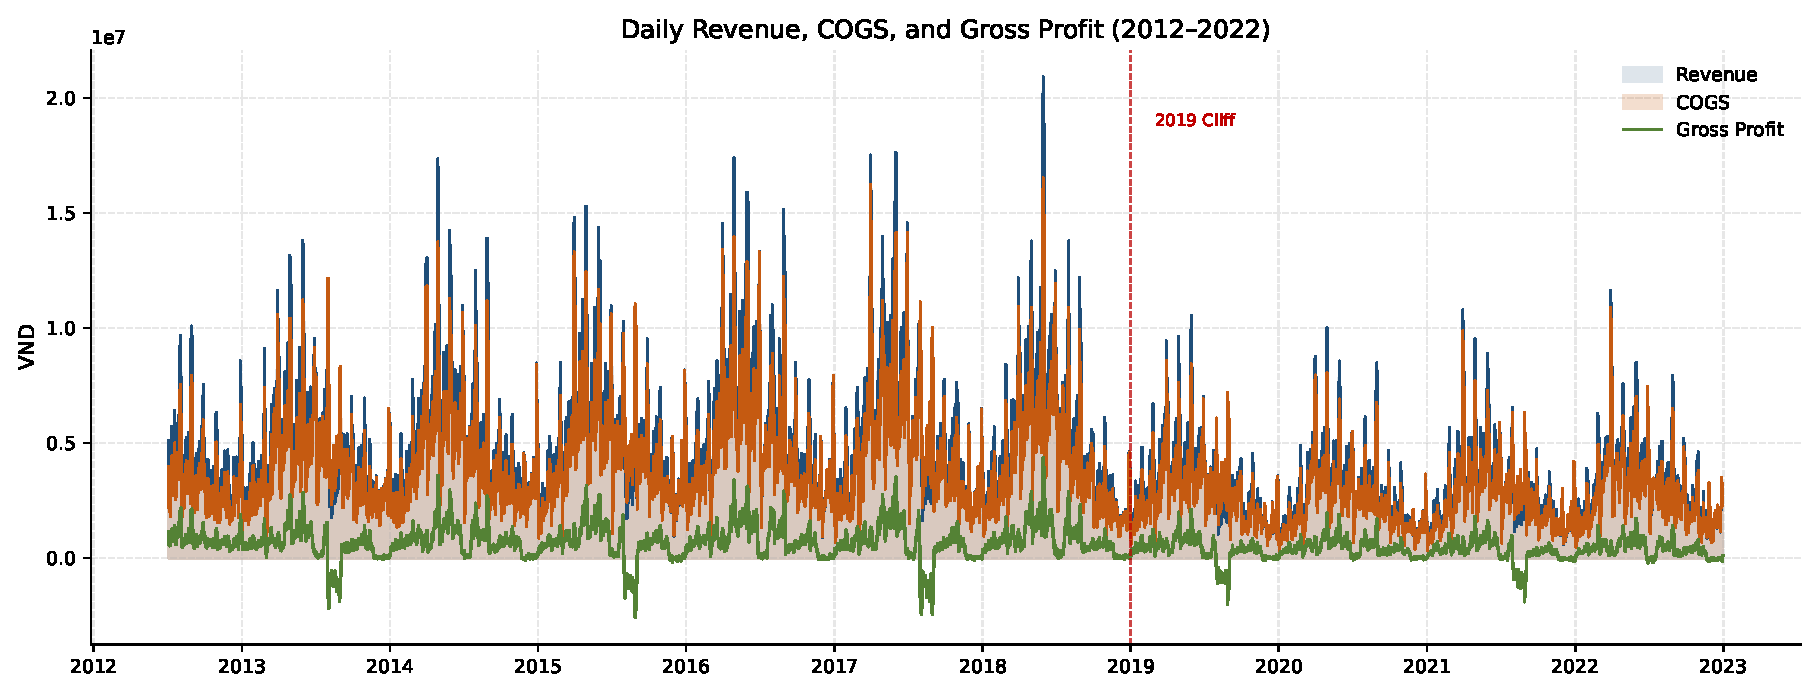
\includegraphics[width=0.85\linewidth]{figures/fig01_revenue_cogs_profit}
  \caption{Daily Revenue, COGS, and Gross Profit (2012--2022). The 2019 structural break is marked by the red dashed line.}
  \label{fig:revenue}
\end{figure}

\textbf{Why it happened (Diagnostic).} The broken lever is session-to-order conversion: it collapsed from 1.17\% (2013) to 0.31\% (2022) -- a $-73\%$ decline. AOV rose from 21,564 to 32,489 VND ($+51\%$), providing a partial buffer but insufficient to offset the order-volume decline. Figure~\ref{fig:demand_capture} (left) visualises this divergence: bars for orders and a line for sessions moving in opposite directions.

Two operational drags compound the conversion problem. First, the \textbf{device blind spot}: tablet converts at only 0.11\%, one-third the mobile rate (Figure~\ref{fig:demand_capture}, right). The ``mobile-first'' assumption is half-right; the real leak is tablet UX. Second, the \textbf{COD tax}: COD orders cancel at 16.0\% versus 8.0\% for prepaid -- a 2$\times$ structural tax, driven by trust friction rather than purchasing power (AOV is nearly identical at $\approx$25,400 VND).

\begin{figure}[t]
  \centering
  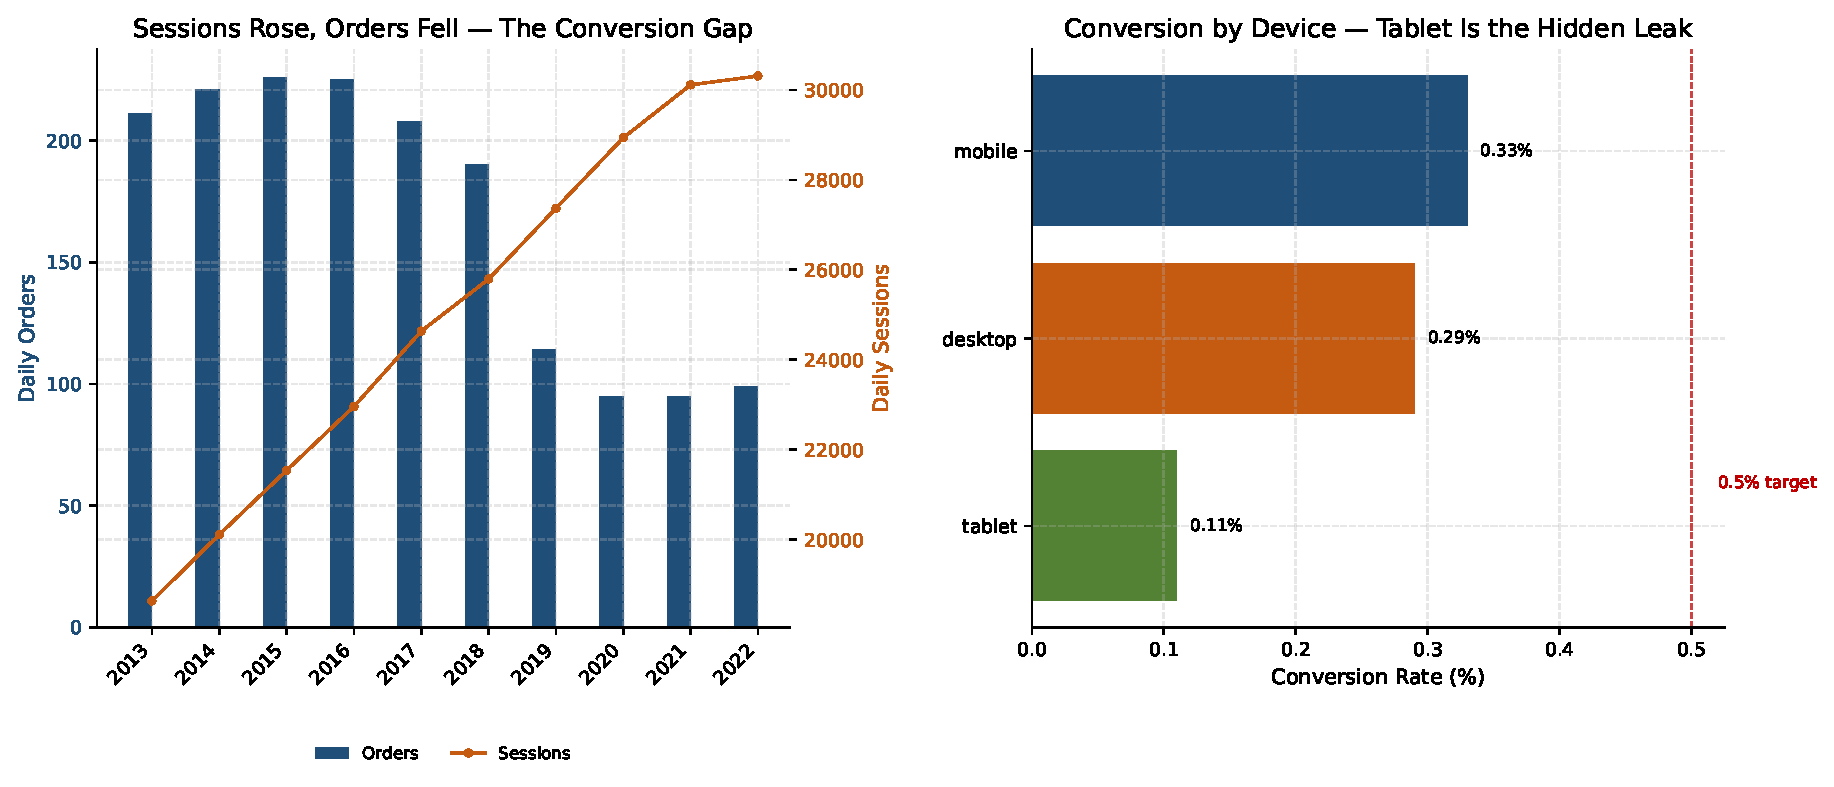
\includegraphics[width=0.85\linewidth]{figures/fig02_demand_capture}
  \caption{(Left) Sessions rose while orders stagnated -- the funnel leaks at the bottom. (Right) Tablet converts at one-third the mobile rate.}
  \label{fig:demand_capture}
\end{figure}

Customer economics compound the treadmill. Month-1 cohort retention is only 3.6\%; for every 1,000 first-time buyers, only 36 return within 30 days. The top 10\% of customers generate 40\% of revenue, and the top 20\% generate 61\% (Figure~\ref{fig:retention}). The business is running an acquisition treadmill with no retention flywheel: organic search drives the most volume but ranks last on efficiency, while Direct -- the smallest channel -- delivers the highest LTV and lowest churn.

\begin{figure}[t]
  \centering
  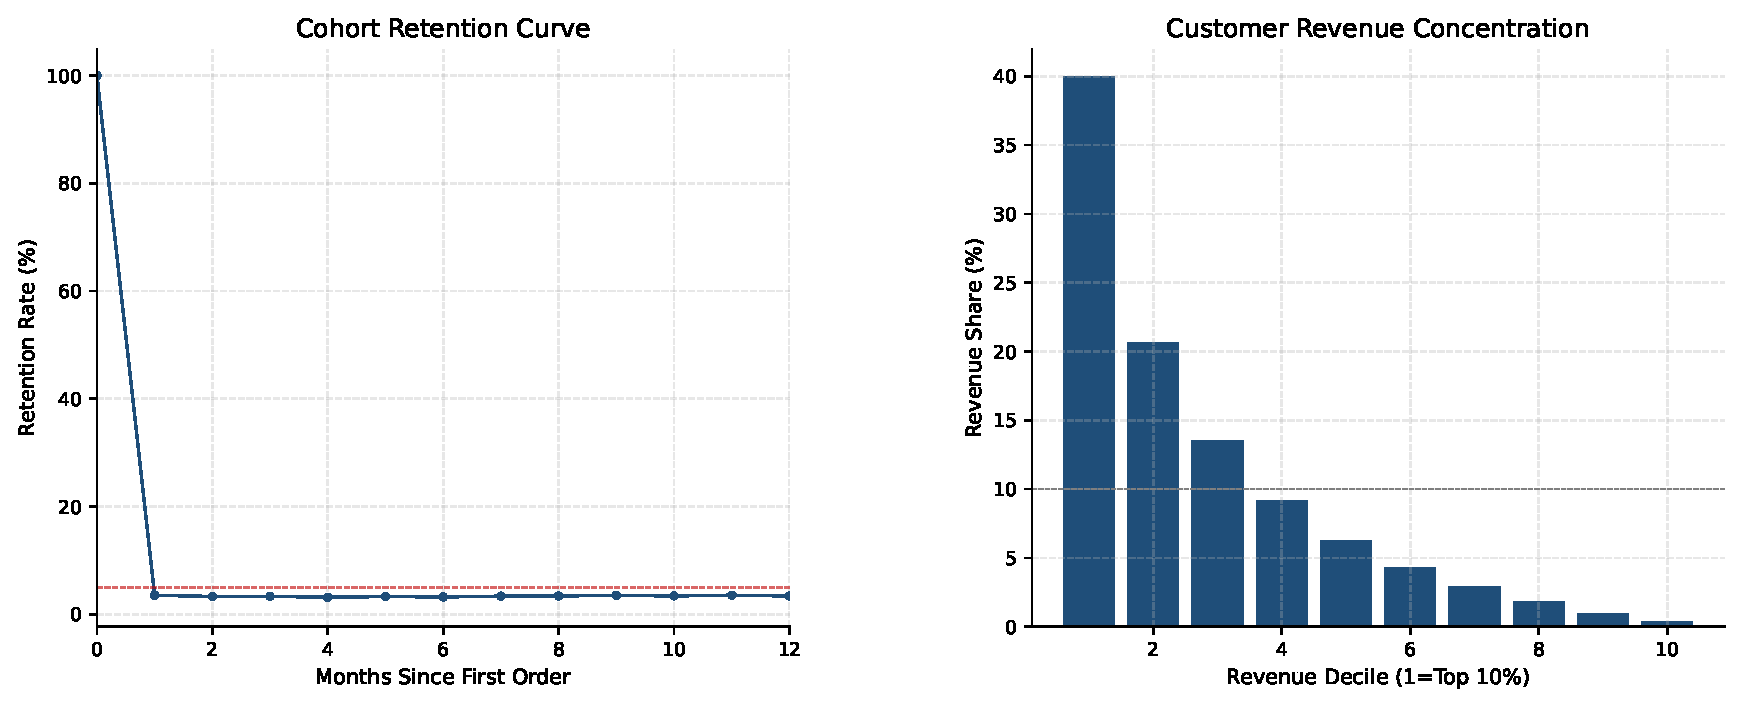
\includegraphics[width=0.85\linewidth]{figures/fig06_retention_clv}
  \caption{(Left) Cohort retention curve -- 96.4\% never return within 30 days. (Right) Top 10\% generate 40\% of revenue.}
  \label{fig:retention}
\end{figure}

\textbf{What is likely next (Predictive).} If the current conversion trajectory continues -- flatlining near 0.3\% -- even aggressive traffic growth will produce diminishing returns. Every new visitor costs marketing budget, but fewer than one in three hundred convert. The customer base will thin at the top while the bottom churns and replaces itself at high acquisition cost.

\textbf{What to do (Prescriptive).} Fix tablet checkout UX first (the true conversion killer, not mobile). A +1pp conversion lift at 2022 traffic adds $\approx$9.9M VND/day ($\approx$3.6B/year) with zero additional marketing spend. Launch a ``first-order credit-card discount'' to cut the COD tax, and shift 10--15\% of organic/paid search budget toward Direct and Referral. For the 22,358 single-order customers, send a ``second purchase incentive'' within 30 days -- the highest-ROI retention lever available.

\subsection{Portfolio, Quality, and Marketing Misalignment}

\textbf{What the data shows (Descriptive).} Streetwear dominates revenue (13.2B VND) but has the lowest margin (13.2\%); GenZ has the highest margin (19.1\%) but the smallest revenue (0.34B VND). The portfolio is drifting toward low-margin volume (Figure~\ref{fig:portfolio_drift}, left). Meanwhile, 814 never-sold SKUs tie up catalog complexity, and inventory bloat sits at 930 days of supply ($\approx$2.5 years) against a 90-day industry standard -- a structural working-capital trap (Figure~\ref{fig:portfolio_drift}, right).

\begin{figure}[t]
  \centering
  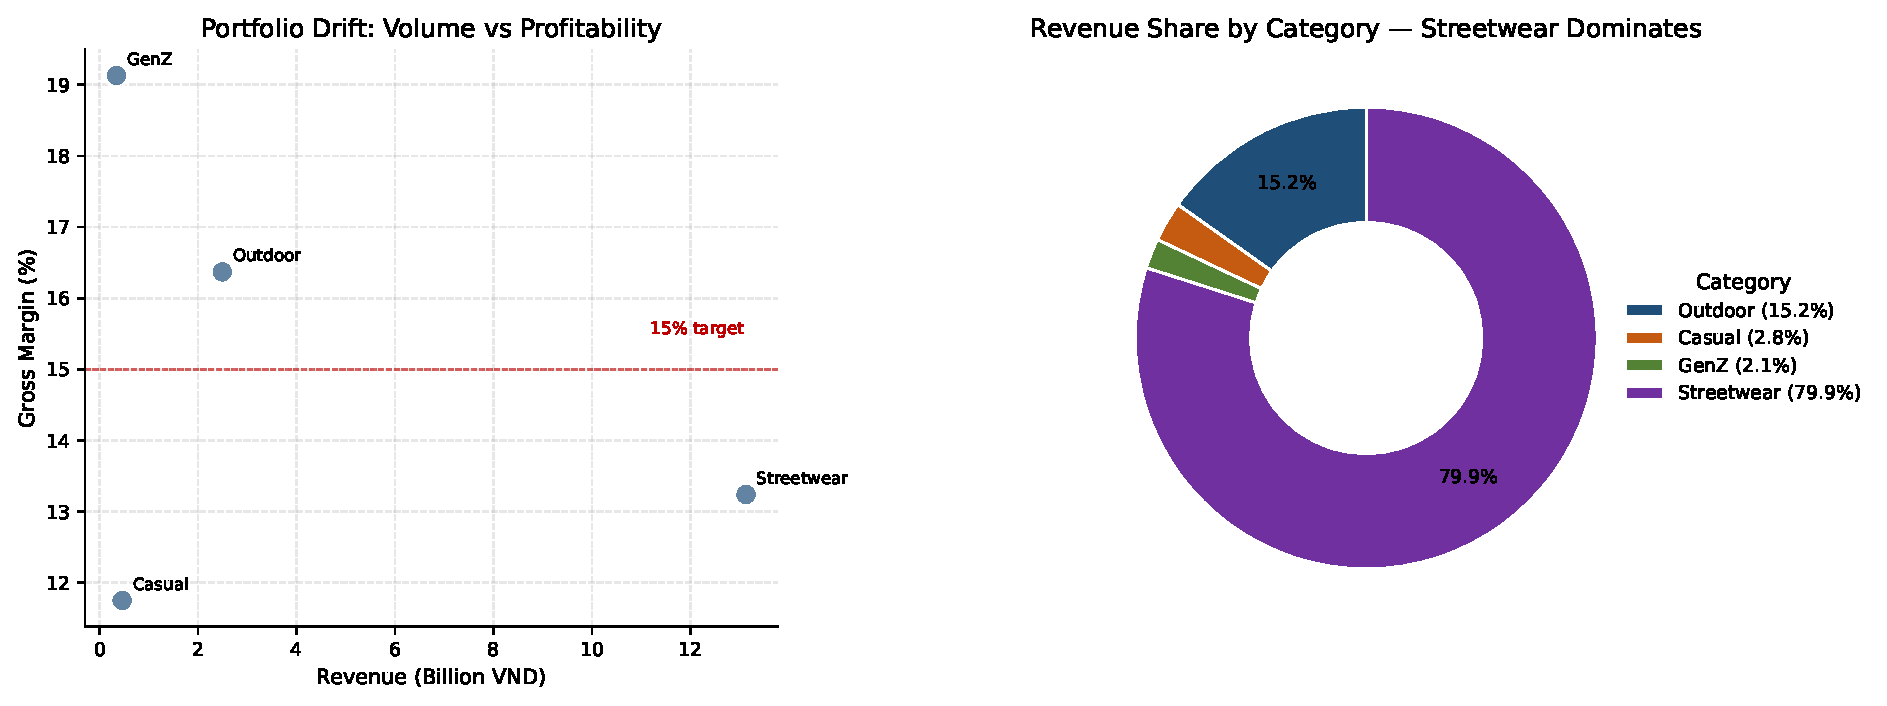
\includegraphics[width=0.85\linewidth]{figures/fig07_portfolio_drift}
  \caption{(Left) Portfolio drift: volume vs profitability by category. (Right) Revenue share confirms Streetwear dominance.}
  \label{fig:portfolio_drift}
\end{figure}

Return rate sits at 5.6\%, persistently above the 5\% alert threshold. The majority are controllable: wrong-size and defective together account for 55\% -- fixable with better sizing guides and supplier QC. West has the highest return rate (3.5\%) despite the lowest revenue, suggesting a product-mix or sizing mismatch rather than a logistics cost problem.

Conventional retail wisdom says Q4 drives peak revenue. For this business, the opposite is true: the peak is April--May (seasonal index 1.56) and the trough is November--December (0.60). The promo mix compounds the misalignment: fixed discounts deliver 79.7$\times$ ROI versus 6.8$\times$ for percentage discounts -- an 11.7$\times$ advantage per discount VND -- yet the business defaults to the less efficient format (Figure~\ref{fig:marketing_misalignment}).

\begin{figure}[t]
  \centering
  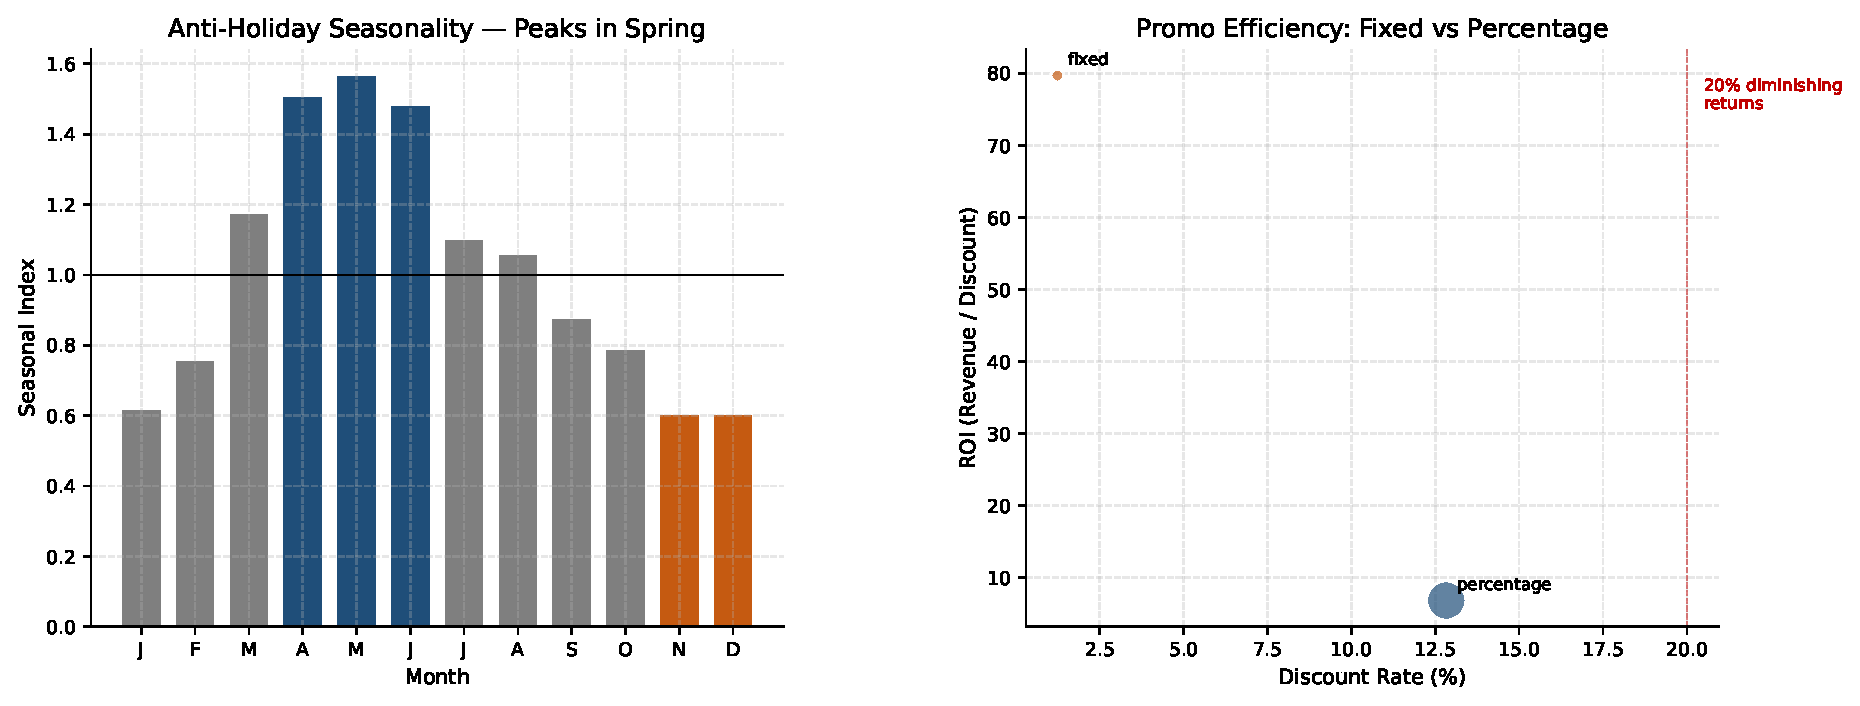
\includegraphics[width=0.85\linewidth]{figures/fig05_marketing_misalignment}
  \caption{(Left) Anti-holiday seasonality -- peaks in spring, troughs in winter. (Right) Fixed discounts deliver 11.7$\times$ the ROI of percentage discounts.}
  \label{fig:marketing_misalignment}
\end{figure}

\textbf{Why it happened (Diagnostic).} The margin crisis is structural, not cyclical. The business has expanded SKU count rather than prioritising active replenishment. Active SKUs generate 2.5$\times$ the revenue per unit as discontinued ones, yet marketing budget chases volume in the wrong category (Streetwear) and the wrong months (Q4). The discount calendar is a ritual with diminishing returns -- percentage promo revenue has declined since 2013 at the same 12.9\% average discount depth.

\textbf{What is likely next (Predictive).} If the portfolio mix continues on its current trajectory, overall gross margin will compress further as Streetwear captures an ever-larger share of incremental revenue. Working capital will remain locked in inventory that turns only once every two years. If Q4 budget concentration and percentage-discount rituals continue, marketing ROI will keep declining.

\textbf{What to do (Prescriptive).} Delist the 814 never-sold SKUs immediately. Right-size inventory to 90 days to free $\approx$3.1B VND in working capital. Shift 10\% of Streetwear marketing share toward GenZ and Casual -- a 10\% shift raises portfolio gross margin by $\approx$0.5pp (+77M VND profit). Reallocate 20\% of Q4 budget to April--May, test fixed-discount campaigns, and cut average percentage discount depth by 2pp. Target: cut controllable returns by 50\% within 6 months through supplier QC and sizing-guide improvements.

\section{Forecasting Pipeline}

We frame forecasting as a direct multi-step regression problem. After pruning redundant and leakage-prone features (correlation $>$ 0.95, stale forward-fill), 35 columns remain: calendar variables, seasonal profiles, promo intensity, and Prophet baselines. Target treatment uses log-residuals (`log1p(revenue) - log\_baseline') so the model learns deviation from seasonality rather than raw level. COGS is modelled sequentially: the revenue model predicts first, and its output is fed into a second COGS model that learns cost conditional on predicted revenue. LightGBM and XGBoost regressors are tuned with Optuna (50 trials) and evaluated on 2-fold sliding-window CV (horizon = 548 days). A spike classifier boosts predictions for high-revenue days.

Table~\ref{tab:cv} reports CV results. The ensemble halves the naive baseline error.

\begin{table}[ht]
  \centering
  \caption{CV Results (2-fold $\times$ 548d horizon)}
  \label{tab:cv}
  \small
  \begin{tabular}{@{}lrrr@{}}
    \toprule
    \textbf{Model} & \textbf{Revenue MAE} & \textbf{COGS MAE} & \textbf{Total MAE} \\
    \midrule
    Seasonal Naive & 1,630,377 & 1,295,990 & 2,926,367 \\
    LightGBM (direct, log-residual) & 821,861 & 758,495 & 1,580,356 \\
    XGBoost (direct, log-residual) & 884,762 & 772,365 & 1,657,127 \\
    Weighted Ensemble & 484,160 & 389,534 & 873,694 \\
    \bottomrule
  \end{tabular}
\end{table}

\textbf{What the model learned (SHAP).} Revenue drivers (Figure~\ref{fig:shap_rev}) are dominated by `days\_to\_month\_end' (salary-cycle effect) and day-of-month profiles, with promos as a secondary lever. COGS drivers (Figure~\ref{fig:shap_cogs}) are led by `promo\_month\_avg\_discount' and `predicted\_revenue' (rank \#3), validating the sequential architecture.

\begin{figure}[t]
  \centering
  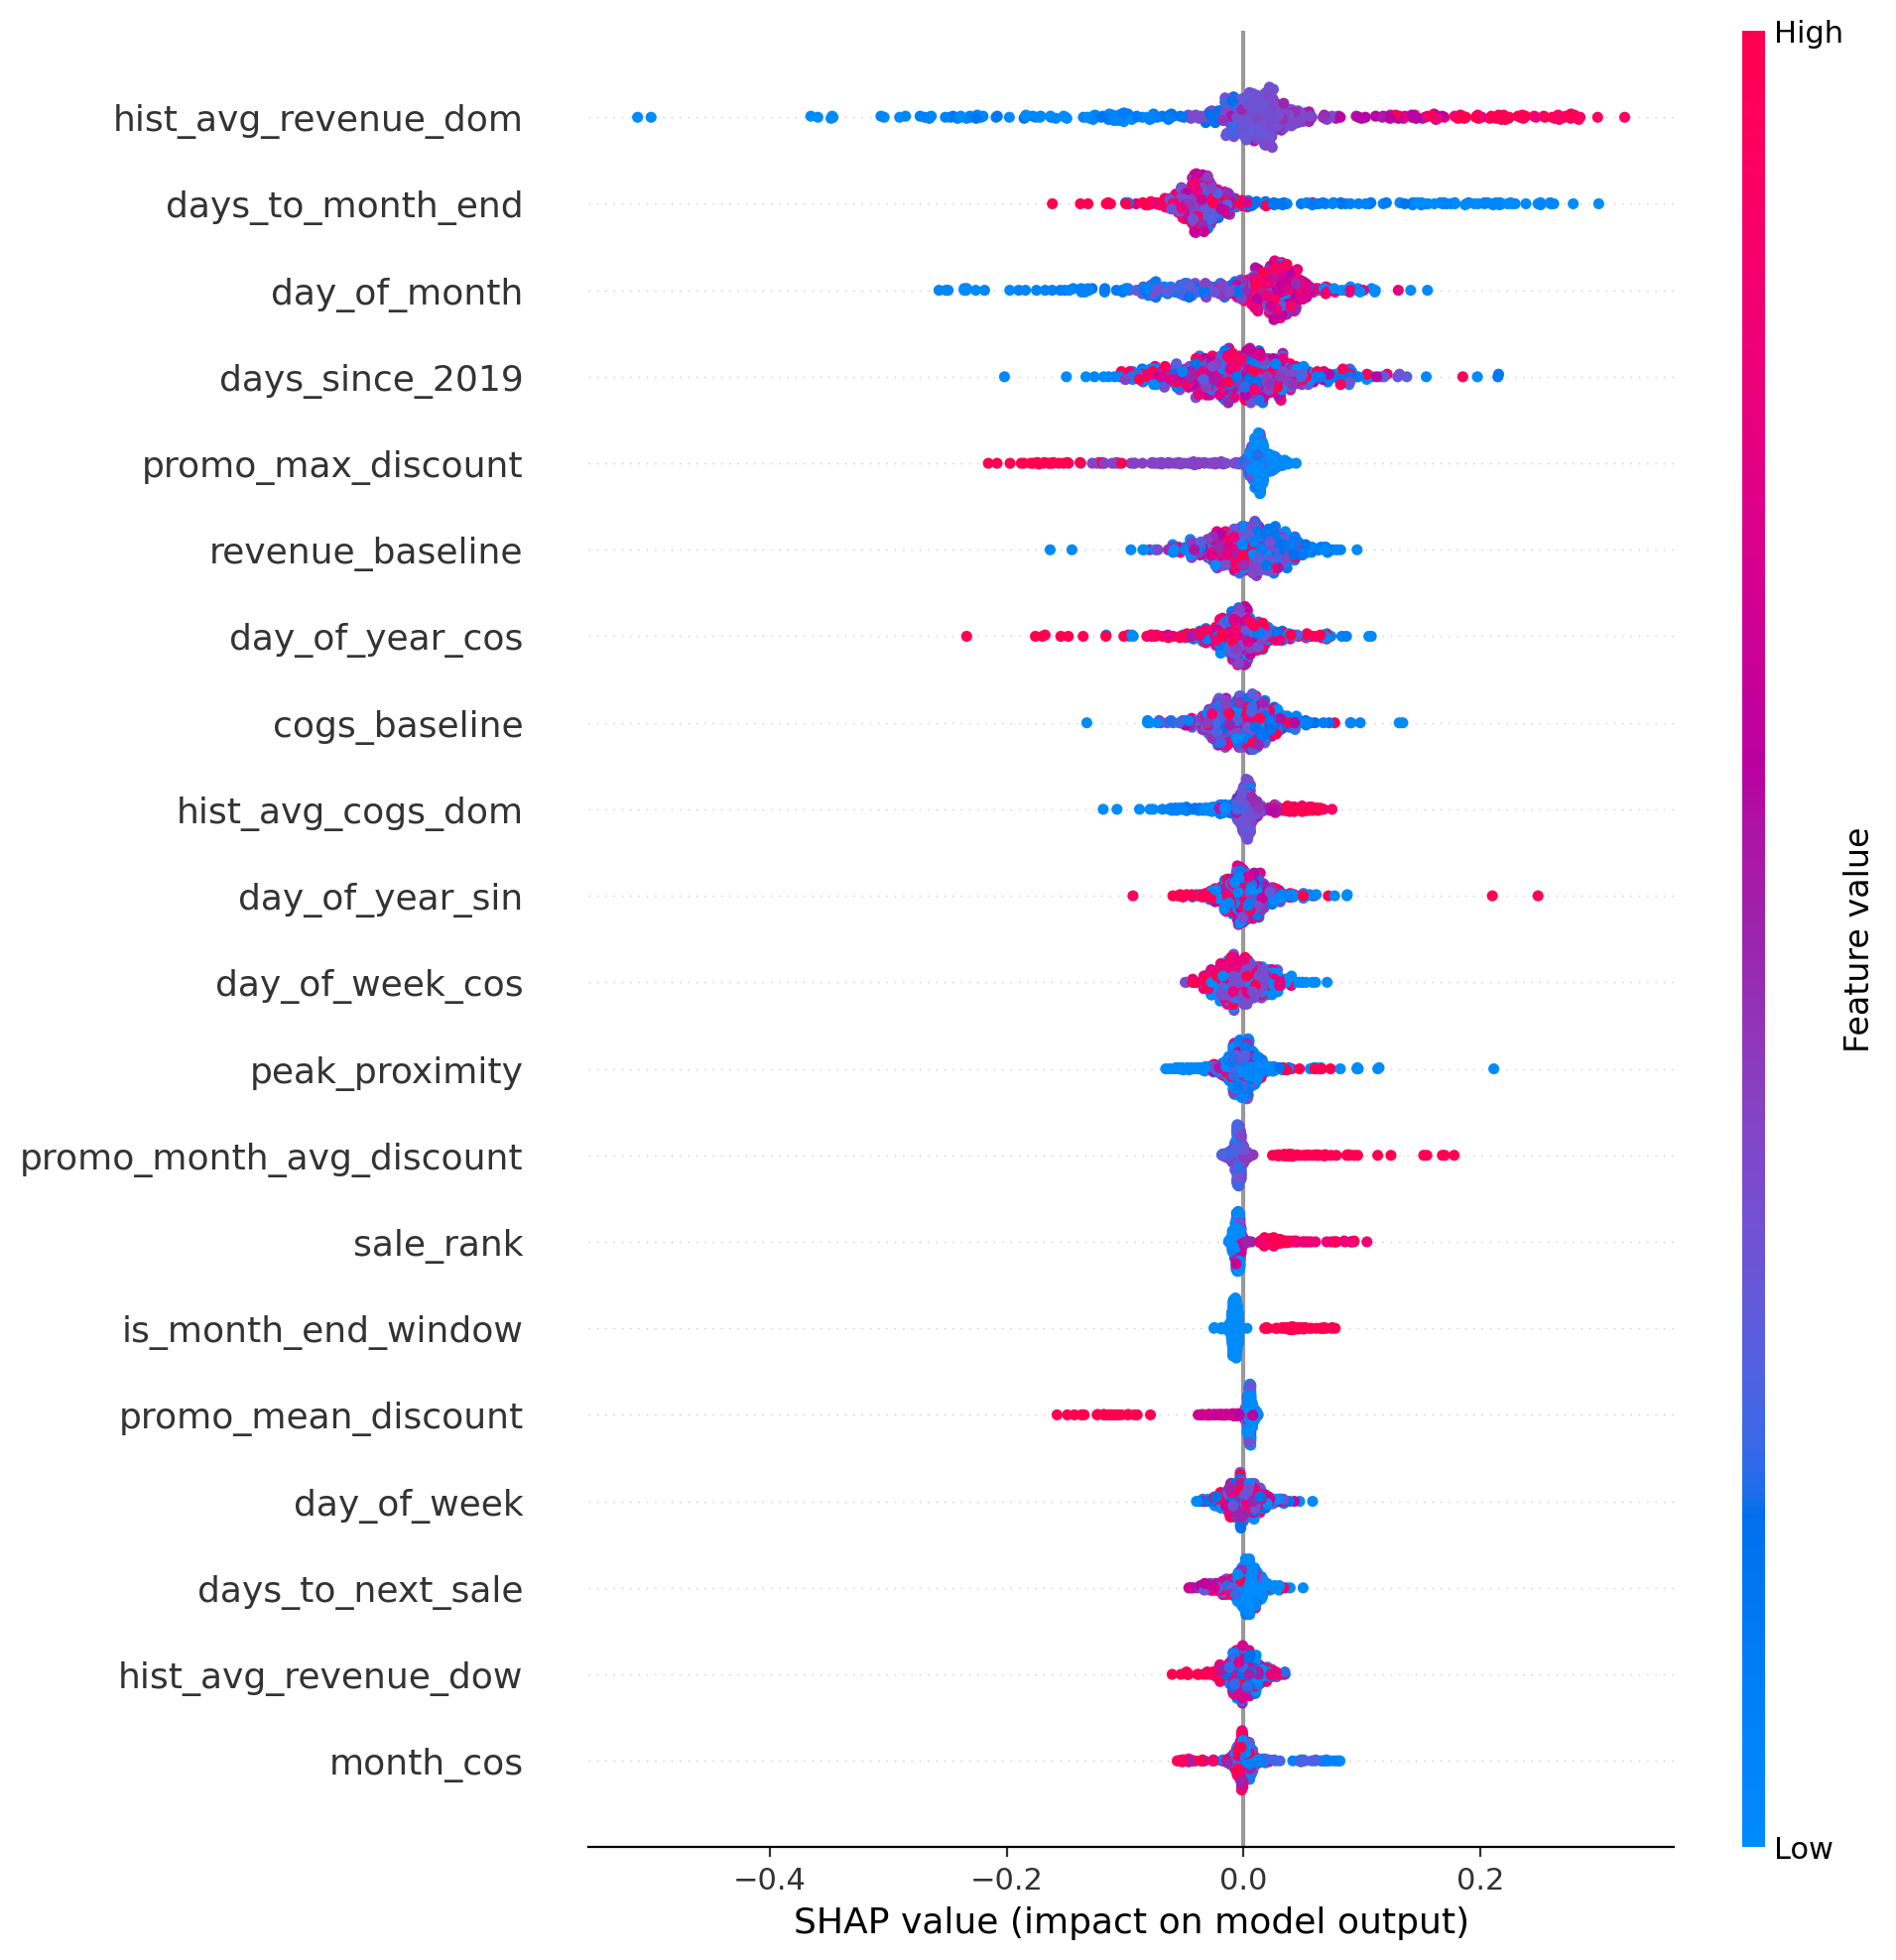
\includegraphics[width=0.85\linewidth]{figures/fig20_shap_revenue}
  \caption{SHAP feature importance for the Revenue model. Salary-cycle and day-of-month profiles dominate; promos are secondary.}
  \label{fig:shap_rev}
\end{figure}

\begin{figure}[t]
  \centering
  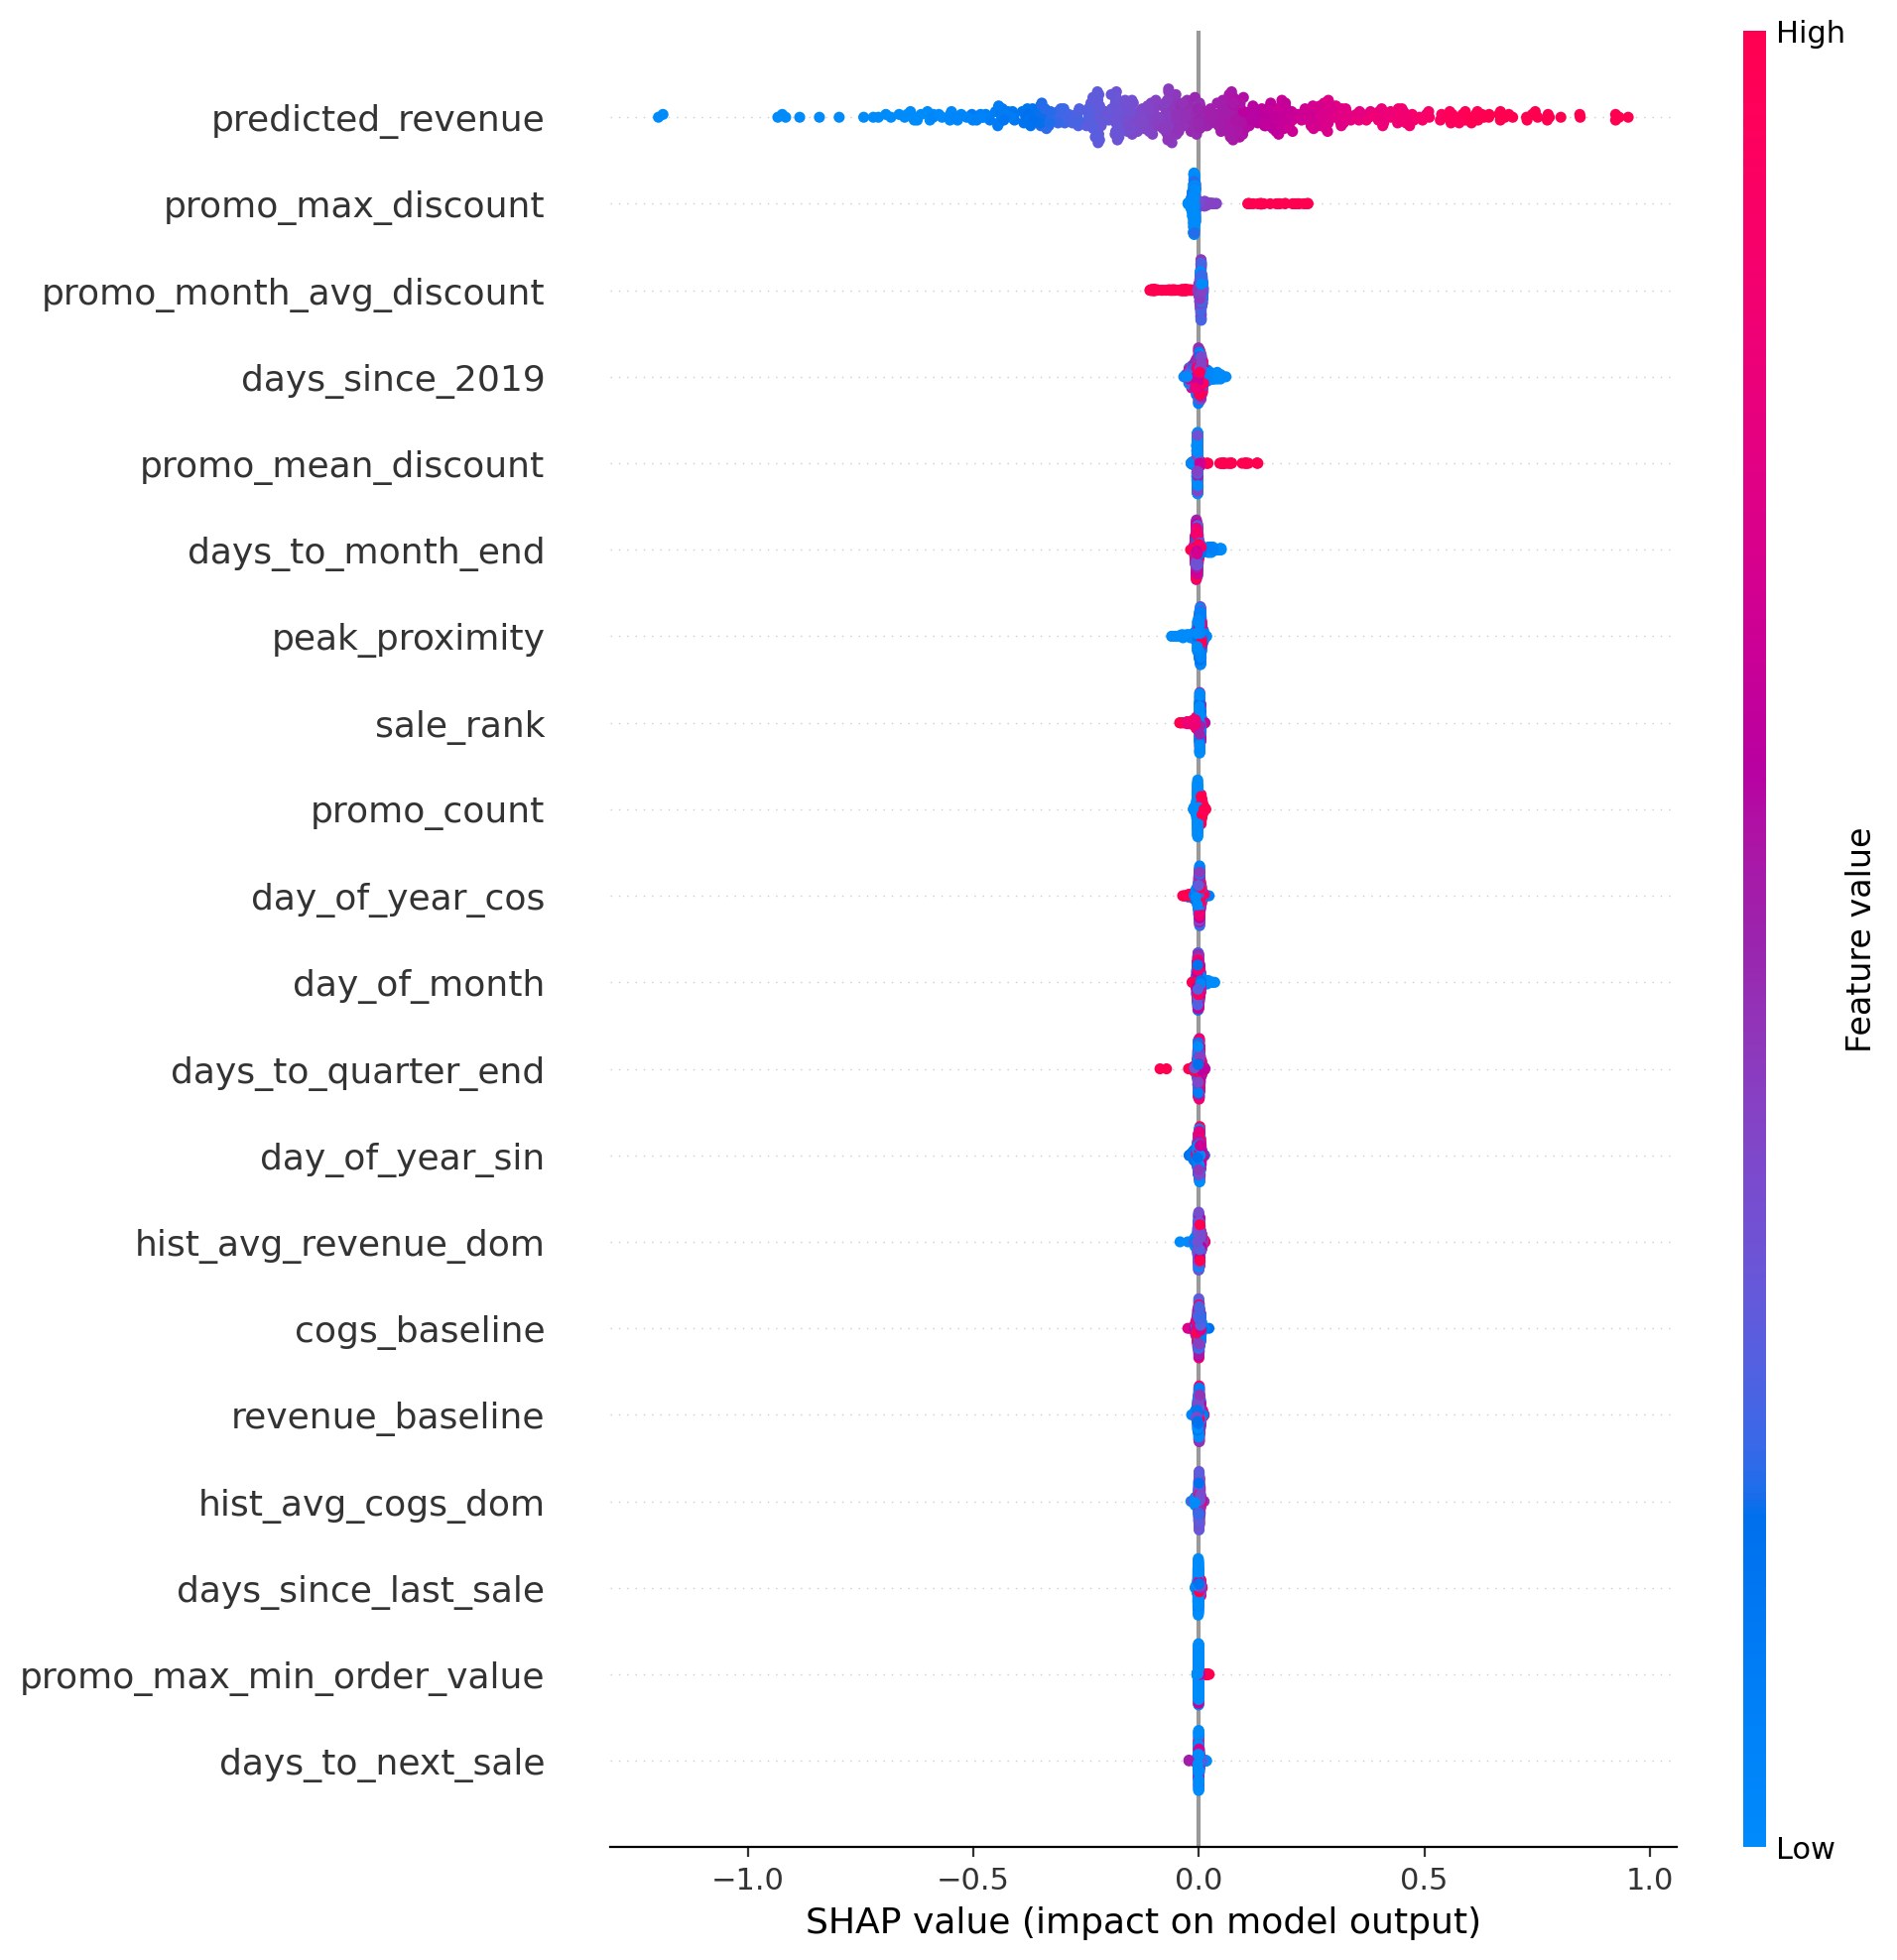
\includegraphics[width=0.85\linewidth]{figures/fig21_shap_cogs}
  \caption{SHAP feature importance for the COGS model. Discount depth is the strongest cost driver; `predicted\_revenue' validates sequential design.}
  \label{fig:shap_cogs}
\end{figure}

\section{Conclusion}

The business is not short of traffic -- it is short of conversion. The 2019 cliff was a structural break in demand capture, not a demand generation failure. Recovery requires fixing tablet checkout UX, re-engaging 22,358 single-order customers, shifting from COD to prepaid to cut the 2$\times$ cancellation tax, and rebalancing the portfolio from low-margin Streetwear volume toward high-margin GenZ quality. The forecasting pipeline provides a data-driven baseline for inventory planning and promotional budgeting over the 548-day horizon. All code is available at \url{https://github.com/ToGiaBaoKDL/datathon-helicopter}.

\clearpage
\bibliography{references}
\bibliographystyle{plainnat}

\end{document}
